\documentclass[tikz,border=10pt]{standalone}
\usetikzlibrary{calc}
\begin{document}
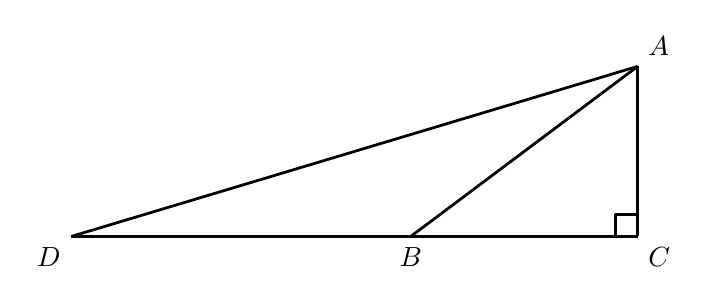
\begin{tikzpicture}[line width=1.0pt, line join=round]
% Pixel -> units: s=0.012214, centre (349,142), y flipped
\coordinate (D) at (-3.554,-1.063);   % px (58,229)
\coordinate (B) at (0.758,-1.063);    % px (411,229)
\coordinate (C) at (3.640,-1.063);    % px (647,229)
\coordinate (A) at (3.640,1.097);     % px (647,52)

% Segments: apex to base points, base D-B-C
\draw (A) -- (D);
\draw (A) -- (B);
\draw (A) -- (C);
\draw (D) -- (B) -- (C);

% Right-angle mark at C (side about 23 px = 0.284 units)
\draw ($(C)+(-0.284,0)$) -- ($(C)+(-0.284,0.284)$) -- ($(C)+(0,0.284)$);

% Labels
\node[above right, font=\fontsize{10}{12}\selectfont] at (A) {$A$};
\node[below, font=\fontsize{10}{12}\selectfont] at (B) {$B$};
\node[below right, font=\fontsize{10}{12}\selectfont] at (C) {$C$};
\node[below left, font=\fontsize{10}{12}\selectfont] at (D) {$D$};
\end{tikzpicture}
\end{document}